\documentclass[11pt,a4paper]{article}
\usepackage[T1]{fontenc}
\usepackage[utf8]{inputenc}
\usepackage{lmodern}
\usepackage{amsmath,amssymb,amsthm,mathtools,mathrsfs}
\usepackage{graphicx,float,xcolor,multicol}
\usepackage[shortlabels]{enumitem}
\usepackage[margin=27mm]{geometry}
\usepackage{microtype,needspace,placeins}
\usepackage{tikz,tikz-cd}
\usetikzlibrary{arrows.meta,calc,positioning,patterns,decorations.pathreplacing}
\usepackage[colorlinks=true,linkcolor=teal,urlcolor=teal,citecolor=teal]{hyperref}
\setlength{\parindent}{0pt}
\setlength{\parskip}{.6em}
\setcounter{secnumdepth}{0}
\allowdisplaybreaks
\raggedbottom
\providecommand{\cross}{\times}
\DeclareUnicodeCharacter{2020}{\ensuremath{\dagger}}
\DeclareMathOperator{\supp}{supp}
\DeclareMathOperator*{\esssup}{ess\,sup}
\providecommand{\chapter}{\section}
\newenvironment{tool}[2]{\subsection*{Tool #1 --- #2}}{}
\newcommand{\ToolRef}[1]{Tool #1}
\newcommand{\FigureTag}[2]{\textit{Figure #1}}
\newcommand{\Result}[1]{\subsection*{#1}}
\newcommand{\Application}[1]{\subsubsection*{Application\if\relax\detokenize{#1}\relax\else\space--- #1\fi}}
\newcommand{\ProofHeading}{\par\textit{Proof.}\space}
\newcommand{\ProofOf}[1]{\par\textit{Proof of #1.}\space}
\newcommand{\RemarkHeading}{\par\textbf{Remark.}\space}
\newcommand{\NoteHeading}{\par\textbf{Note.}\space}
\newcommand{\ExerciseHeading}{\par\textbf{Exercise.}\space}

\graphicspath{{figures/elliptic-curves/}}
\begin{document}
\section*{Elliptic Curves — Geometric Perspective}
% BLOG-CONTENT-BEGIN
Flipping through the pages of math-literature from the late 19th century to the early 21st century one would stumble upon elliptic curves via three distinct routes:-
\begin{itemize}
    \item Geometric Way (genus 1 Riemann surfaces) 
    \item Algebraic Way (smooth cubic curves in $\mathbb{CP}^2$) 
    \item Harmonic Way (modular forms on $\mathbb{H}$)
\end{itemize}
\begin{figure}[!htb]
            \minipage{0.32\textwidth}
                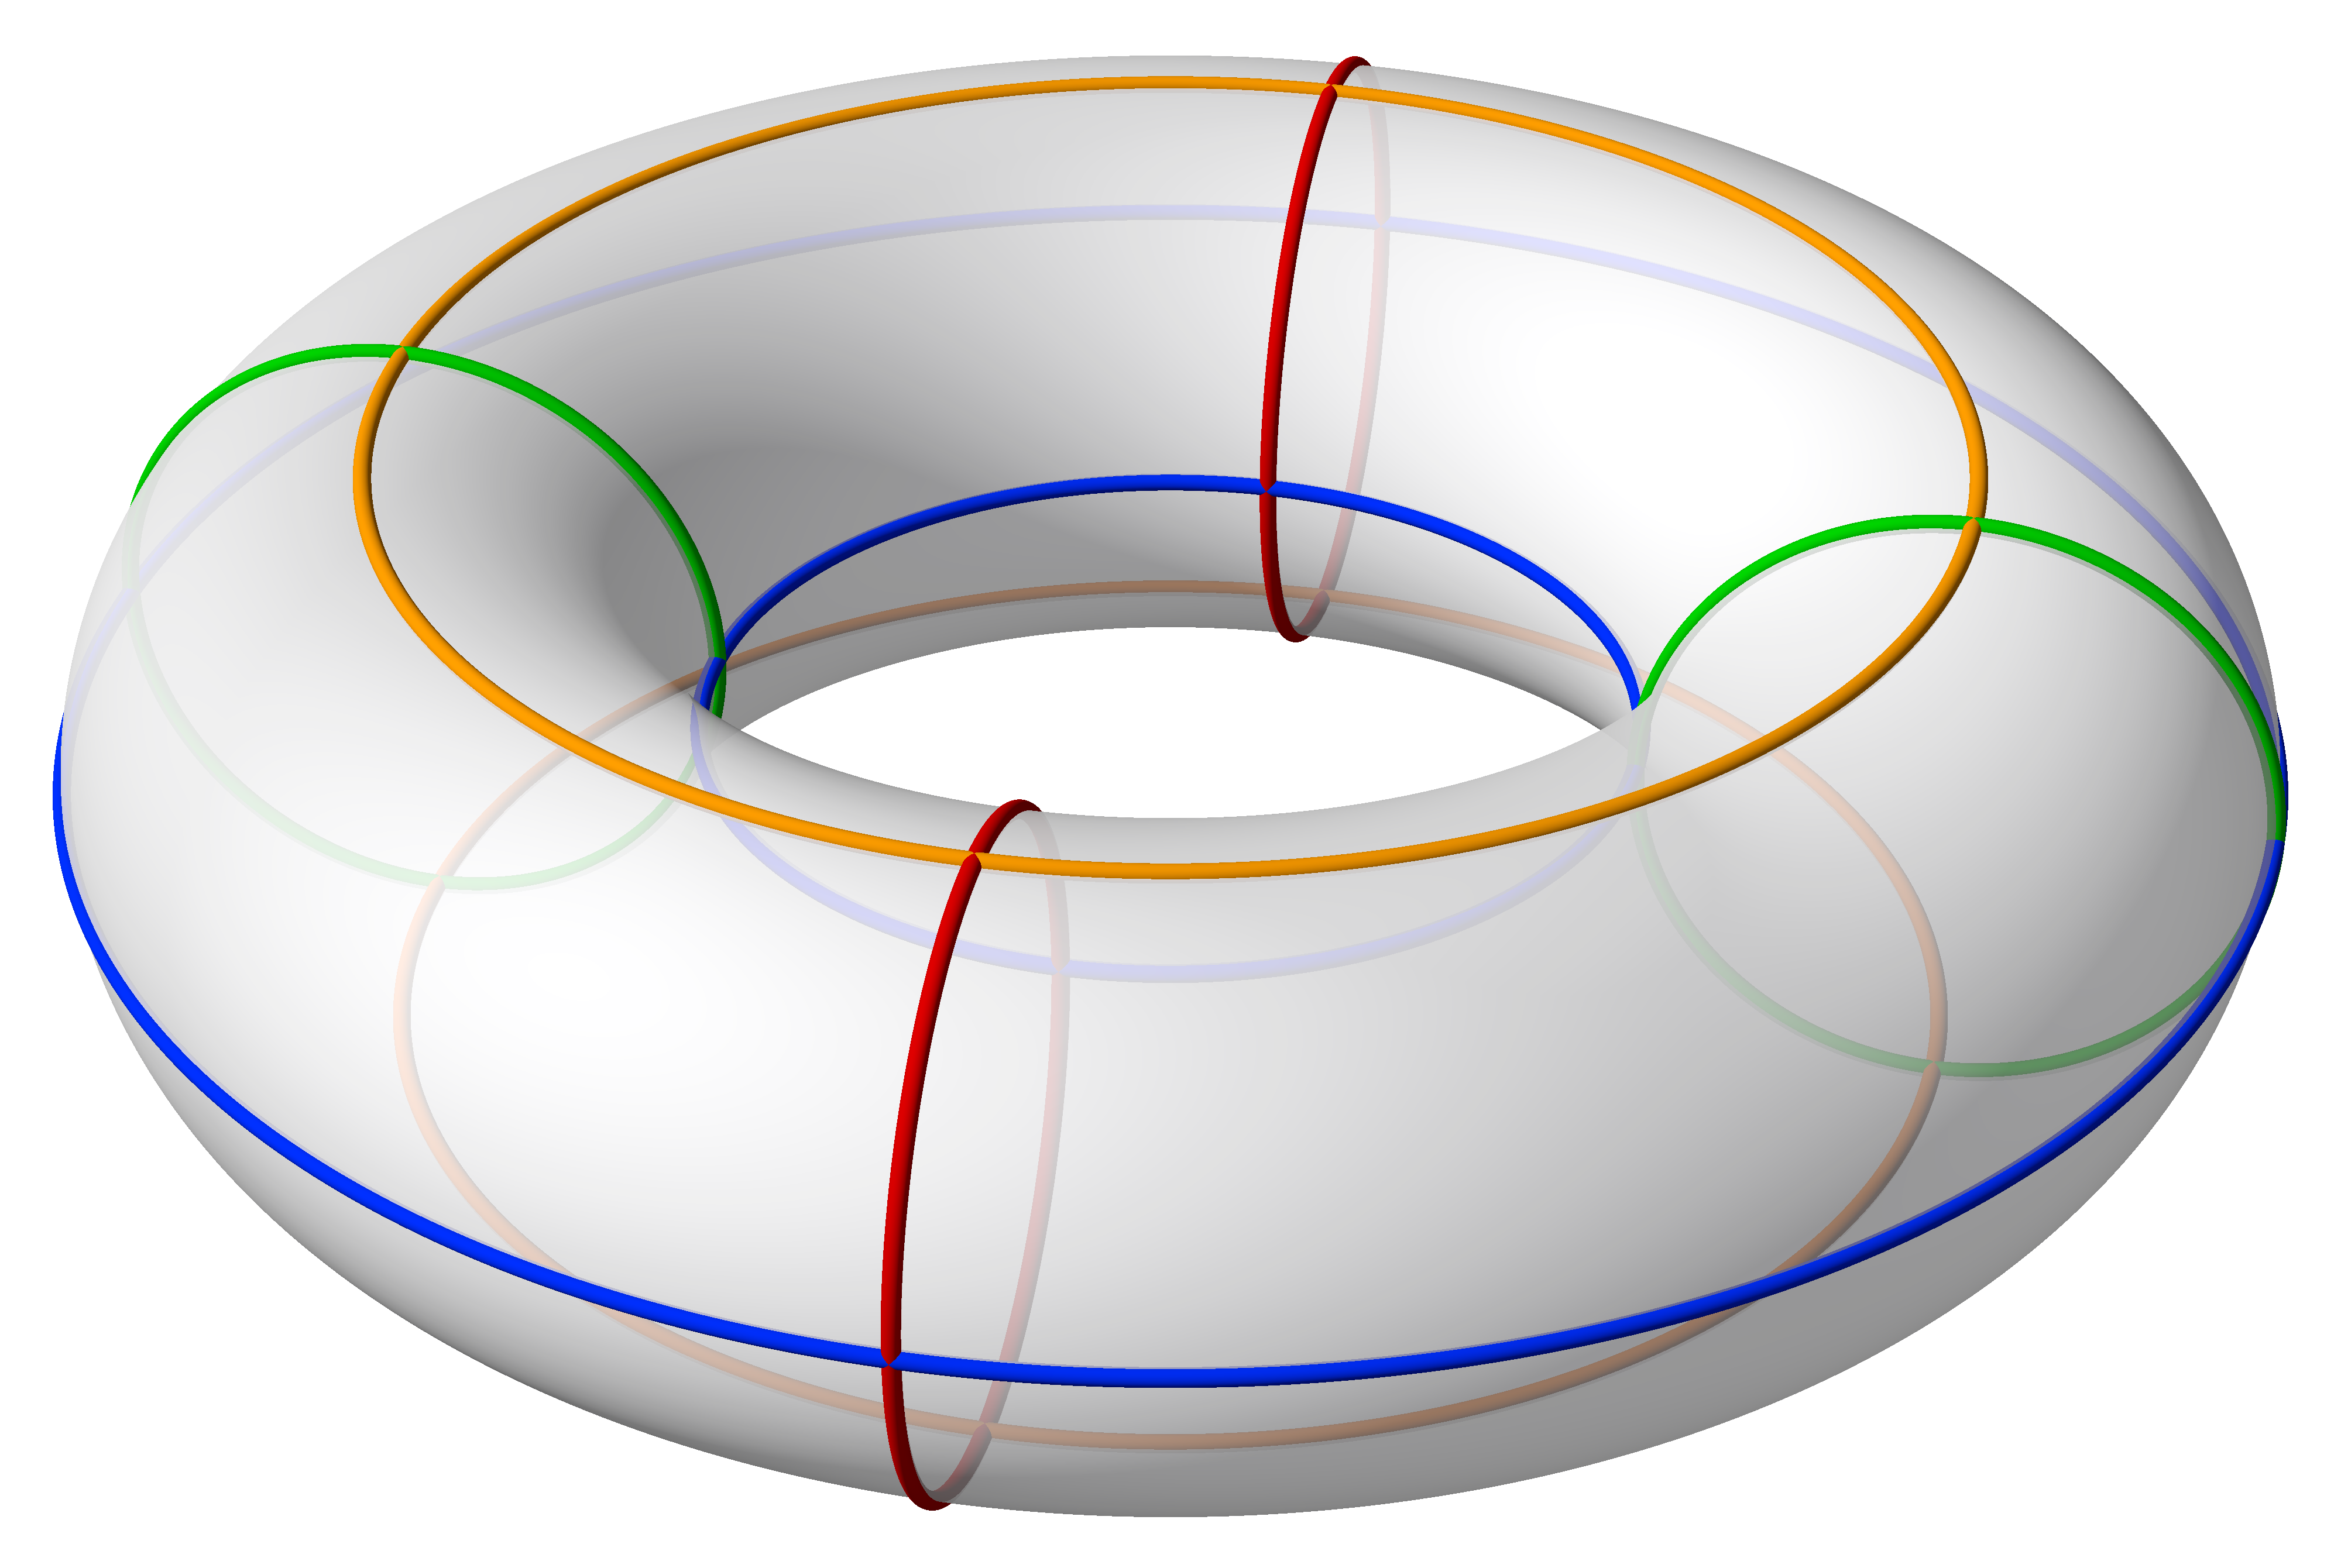
\includegraphics[width=\linewidth]{Torus.png}
                
            \endminipage
            \minipage{0.32\textwidth}
                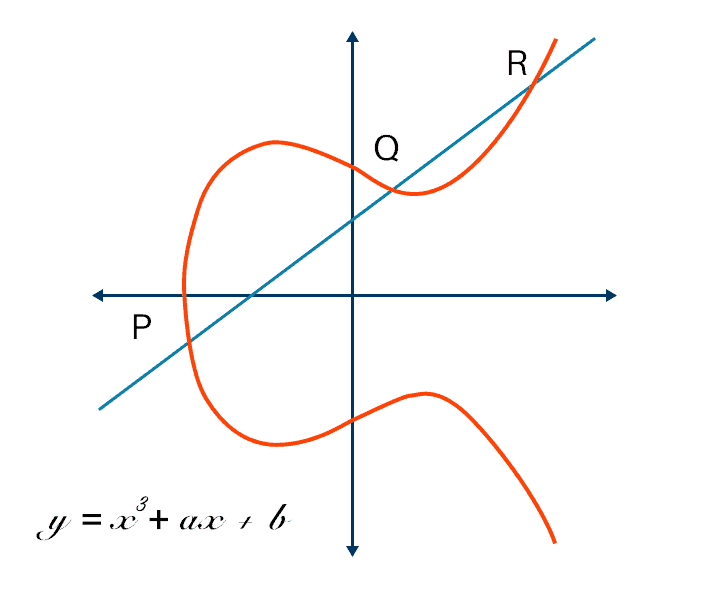
\includegraphics[width=\linewidth]{elliptic curves.png}
                
            \endminipage
            \minipage{0.32\textwidth}
                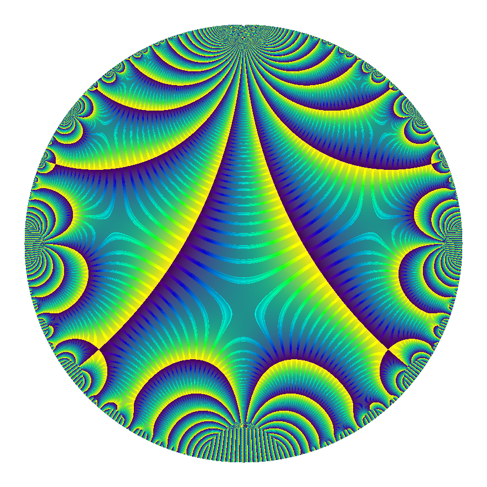
\includegraphics[width=\linewidth]{Modular Forms.png}
                
            \endminipage
        \caption{Different ways of looking at elliptic curves are illustrated pictorially.}
        \end{figure}


Delightful pieces of mathematics emerged out of realizing that the three ways blend into one another seamlessly. We shall outline that in this exposition.

\textbf{I) \underline{Geometric Perspective}}

Uniformization Theorem tells us that a Riemann surface of genus 1 is obtained via $\mathbb{Z}^2$ symmetries of $\mathbb{C}$, (i.e.) they are obtained by a covering space action of the group $\mathbb{Z}^2$ on $\mathbb{C}$. Consider the generators $(0,1)$ and $(1,0)$ of $\mathbb{Z}^2$, we have the following automorphisms:-
$$(0,1): \mathbb{C} \rightarrow \mathbb{C}$$
$$(1,0): \mathbb{C} \rightarrow \mathbb{C}$$
Let $(0,1)(0) = \omega_1$ and $(1,0)(0) = \omega_2$, then $\Lambda := \mathbb{Z}\omega _1 \oplus \mathbb{Z}\omega_2 \subset \mathbb{C}$ is called the lattice associated to the $\mathbb{Z}^2$ action $\alpha$ on $\mathbb{C}$, and the surface that $\alpha$ yields shall be denoted by $\mathbb{C}/\Lambda$. Topologically speaking all surfaces $\{\mathbb{C}/\Lambda\}_{\Lambda \in \text{lattices}}$ are equivalent to a torus ($\mathbb{S}^1\times \mathbb{S}^1$) given by the following well-known polygonal representation.  

\begin{center}
   \tikzset{every picture/.style={line width=0.75pt}}
\begin{tikzpicture}[x=0.75pt,y=0.75pt,yscale=-1,xscale=1]



\draw   (264.7,50) -- (460,50) -- (376.3,219.5) -- (181,219.5) -- cycle ;
\draw   (280.5,215.5) -- (290.5,219.75) -- (280.5,224) ;
\draw   (341,45) -- (352,50.25) -- (341,55.5) ;
\draw   (236.2,120.39) -- (226.04,127.2) -- (224.85,115.03)(234.49,124.01) -- (224.33,130.82) -- (223.14,118.64) ;
\draw   (427.92,128.88) -- (417,136.64) -- (417.19,123.25)(426.06,132.42) -- (415.14,140.19) -- (415.33,126.79) ;


\draw (245,28.4) node [anchor=north west][inner sep=0.75pt]    {$\omega _{1}$};

\draw (165,219.4) node [anchor=north west][inner sep=0.75pt]    {$0$};

\draw (373,225.4) node [anchor=north west][inner sep=0.75pt]    {$\omega _{2}$};

\draw (455,28.4) node [anchor=north west][inner sep=0.75pt]    {$\omega _{1} +\omega _{2}$};

\draw (198,119.4) node [anchor=north west][inner sep=0.75pt]    {$\alpha $};

\draw (344,18.4) node [anchor=north west][inner sep=0.75pt]    {$\beta ^{-1}$};

\draw (281,231.4) node [anchor=north west][inner sep=0.75pt]    {$\beta $};

\draw (431,124.4) node [anchor=north west][inner sep=0.75pt]    {$\alpha ^{-1}$};


\end{tikzpicture} 
\end{center}

To be in a position to identify these tori as analytic surfaces we must first learn to tell them apart, (i.e.) we must understand morphisms between them.

\subsection*{Theorem 0.1} The following are in bijective correspondence:-
\begin{enumerate}[(i)]
    \item Elements of the modular group $PSL_2(\mathbb{Z})$.
    \item Lattice preserving biholomorphisms between $\big(\mathbb{C}/\Lambda, [\Lambda]\big)$, where $\Lambda$ is generated by $1$, and $\tau \in \mathbb{H}$.
\end{enumerate}

\textit{Proof.}
Let, 
$$\Phi: \big(\mathbb{C}/\Lambda, [\Lambda]\big) \rightarrow \big(\mathbb{C}/\Lambda', [\Lambda']\big)$$
be a lattice preserving holomorphic map, then consider the following diagram:-

\[\begin{tikzcd}
	{\mathbb{C}} & {\mathbb{C}} \\
	{\mathbb{C}/\Lambda} & {\mathbb{C}/\Lambda'}
	\arrow["{p_{\Lambda}}"', from=1-1, to=2-1]
	\arrow["{\widetilde{\Phi}}", dashed, from=1-1, to=1-2]
	\arrow["{p_{\Lambda}}", from=1-2, to=2-2]
	\arrow["\Phi"', from=2-1, to=2-2]
\end{tikzcd}\]

$p_{\Lambda}$ and $p_{\Lambda'}$ are covering maps, and $\mathbb{C}$ being simply-connected lifts $\Phi$ to $\widetilde{\Phi}$. For a fixed $\lambda \in \Lambda$, by construction, $\widetilde{\Phi}(z+\lambda) - \widetilde{\Phi}(z) \in \Lambda'$. Since $\mathbb{C}$ is connected, $\widetilde{\Phi}(z+\lambda) - \widetilde{\Phi}(z) = \lambda'$. Hence, $\widetilde{\Phi}'(z)$ is a doubly periodic entire function, (i.e.) a constant by Liouville's Theorem. As a result, $\widetilde{\Phi}(z) = cz$ such that $c\Lambda \subseteq \Lambda'$. So, morphisms between $\mathbb{C}/\Lambda$ correspond to $\mathbb{Z}$-module morphisms between $\Lambda$. 

Now, if $\Phi$ were an isomorphism, then let $\widetilde{\Phi} \equiv c_1z$ and $\widetilde{\Phi}^{-1} \equiv c_2z$. Clearly, $c_1c_2 = 1$, and we have the following chain of inclusions:-
$$\big(c_1\Lambda \subseteq \Lambda' \subseteq c_2^{-1}\Lambda = c_1\Lambda\big) \implies \big(c_1\Lambda = \Lambda'\big)$$

Now for all pointed surfaces we choose a representative $\big(\mathbb{C}/\Lambda_0, [\Lambda_0]\big)$ such that $\Lambda_0 = \mathbb{Z}\oplus \mathbb{Z}\tau$ (for $\tau \in \mathbb{H}$) (this can be arranged post relevant reflection, rotation, and scaling). An isomorphism,
$$\Phi: \big(\mathbb{C}/\Lambda_0, [\Lambda_0]\big) \rightarrow \big(\mathbb{C}/\Lambda'_0, [\Lambda'_0]\big)$$
corresponds to, 
$$\Psi : \mathbb{Z}\oplus \mathbb{Z}\tau \rightarrow \mathbb{Z}\oplus \mathbb{Z}\tau'$$
$$\Psi(\alpha) := c\alpha$$
This implies, 
$$c\cdot \text{Id}_{2\times 2} \begin{pmatrix}1\\ \tau
\end{pmatrix} = \begin{pmatrix}p\tau' +q\\ r\tau' +s
\end{pmatrix}$$
giving us, 
$$\tau = \frac{p\tau' +q}{r\tau' +s}$$
Every $\Phi$ corresponds uniquely to a $\Psi$, which corresponds to a $GL_2(\mathbb{Z})$ action on $\tau'$, which in turn (by the equation above) admits invariance under the action of scalar matrices. So, $\Phi$ uniquely corresponds to an element in $GL_2(\mathbb{Z})/\big(\lambda\cdot\text{Id}_{2\times 2}\big) = PSL_2(\mathbb{Z})$. One can now trace one's steps back to finish the proof.


\textbf{Remark.} Consider $\phi \in \text{Aut}\big(\mathbb{C}/\Lambda, [\Lambda]\big)$, and $\widetilde{\phi} \equiv cz$ with $c\Lambda = \Lambda$. Note that, $1, c, c^2, \ldots \in \Lambda$,  implying $c$ to be a root of unity for $\Lambda$ is discrete. If $\text{ord}(c) \neq 2,4,6$, assuming WLOG that $c$ is a primitive root, $c^2 \notin \mathbb{Z}$-span of $1$ and $c$. Therefore $\text{Aut}(E, O)$ is one of the three cyclic groups $\mathbb{Z}/2\mathbb{Z}$, $\mathbb{Z}/4\mathbb{Z}$, $\mathbb{Z}/6\mathbb{Z}$.

\begin{figure}[htp]
            \centering
            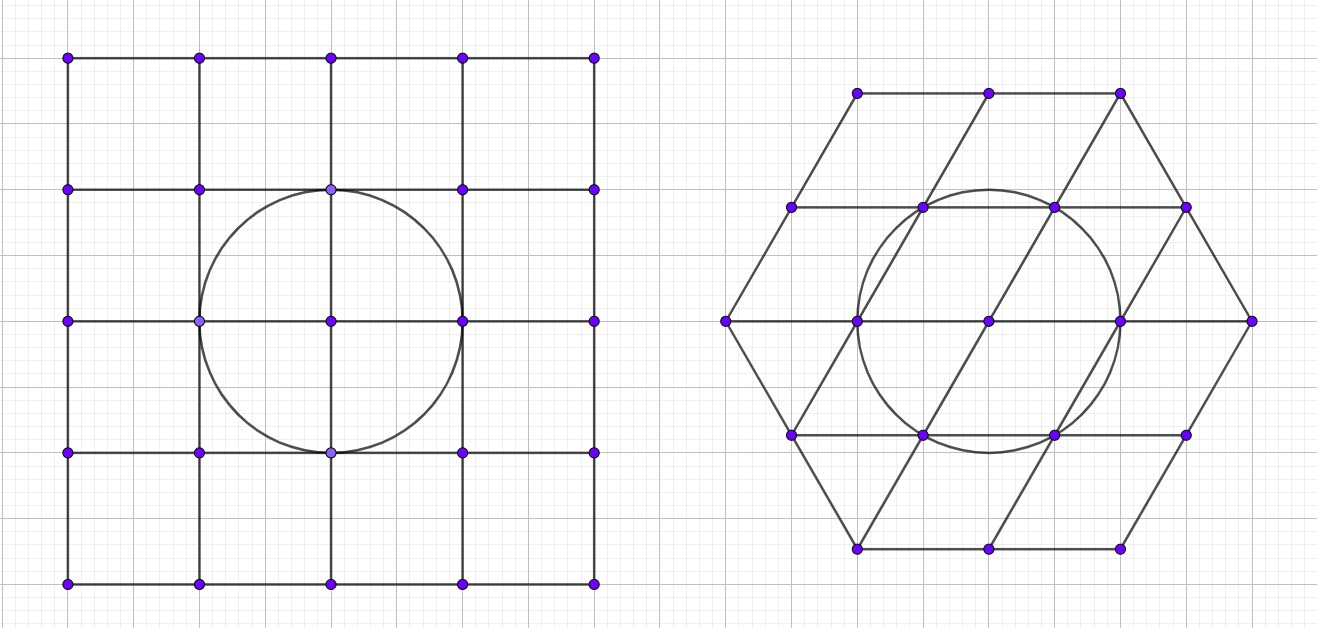
\includegraphics[width=15cm]{Lattices.jpg}
            \caption{The case $\text{ord}(c) = 2,4$ is shown in the left, while on the right one has the triangular lattice for which $\text{ord}(c) = 6$.}
        \end{figure}

So, the theorem above shows that one can tell apart elliptic curves via the shape of the polygon in its polygonal representations upto a $PSL_2(\mathbb{Z})$ symmetry on $\mathbb{H}$. Hence the space $\mathbb{H}/PSL_2(\mathbb{Z})$ can be assigned to keep track of pointed elliptic curves (upto equivalence) - such a space for a class of geometric objects is called it's \textbf{moduli space}. 

From a geometric point of view we understand the nature of pointed complex tori. Let us now acquaint ourselves with families of such surfaces, and for that the following theorem would come in handy.

\subsection*{Theorem 0.2}
    The domain, 
    $$D:= \{z\in \mathbb{H}   |   |\text{Re}(z)| <1/2,   |z|>1\}$$
    maps injectively into $\mathbb{H}/PSL_2(\mathbb{Z})$ such that $\overline{D} \rightarrow \mathbb{H}/PSL_2(\mathbb{Z})$ is surjective. (such domains associated to a group are called \textbf{fundamental domains}, and $PSL_2(\mathbb{Z})$ is suggestively called the \textbf{modular group}).

\textit{Proof.}
    We shall prove the two assertions in the theorem above separately.

    \underline{Injectivity}:- Let $z\in D$ and $\begin{pmatrix}
        a&b\\c&d
    \end{pmatrix} \in PSL_2(\mathbb{Z})$. If $c=0$, $ad = 1$, $a$ and $d$ being integers would force the action to be $g: z\rightarrow z\pm b$. So clearly, $g(z) \notin D$. Now suppose $c\neq 0$, then the action is given by $g: z\rightarrow \frac{az+b}{cz+d}$, which can be rewritten as follows,
    $$\frac{c(az+b)}{c(cz+d)} = \frac{acz +ad - (ad-bc)}{c(cz+d)} = \frac{a(cz+d) - 1}{c(cz+d)} = \frac{a}{c} - \frac{1}{c(cz+d)}$$
    If $z, g(z) \in D$, then, 
    $$\bigg(\frac{\sqrt{3}}{2}\bigg)\bigg(\frac{\sqrt{3}}{2}\bigg) \leq \bigg|g(z) - \frac{a}{c}\bigg|\cdot\bigg|z+\frac{d}{c}\bigg| = \frac{1}{c^2}$$
    forcing $|c| \leq \frac{2}{\sqrt{3}}$, so, $c = \pm 1$. But this implies, 
    $$|g(z)\mp a|\cdot |z\pm d| >1$$
    Contradiction.

    \underline{Surjectivity}:- Let $z \in \mathbb{H}$, $T: z\rightarrow z+1$, and $R: z\rightarrow -1/z$. Choose an element $g'$ from the group generated by $T$ and $R$ for which Im$(g'(z))$ is maximal, then,
    $$\text{Im}(g'(z)) \geq \text{Im}\bigg(\frac{-1}{g'(z)}\bigg) = \frac{\text{Im}(g'(z))}{|g'(z)|^2}$$
    would make $|g'(z)| \geq 1$. Evidently there exists an integer $k$ such that $|\text{Re}(T^k(g'(z))|\leq 1/2$. Note that $T^k(g'(z)$ would retain the optimality of the imaginary part, forcing $|T^k(g'(z)| \geq 1$ to still hold. This would establish surjectivity, for all orbits hit $\overline{D}$ atleast once. It remains to see why such a maximal $g'$ exist. Let $g$ represent the action corresponding to $\begin{pmatrix}
        a&b\\c&d
    \end{pmatrix} \in PSL_2(\mathbb{Z})$, we have,
    $$\text{Im}(gz) = \text{Im}\bigg(\frac{az+b}{cz+d}\bigg) = \text{Im}\bigg(\frac{(az+b)(\overline{cz+d})}{|cz+d|^2}\bigg) = \text{Im}\bigg(\frac{ac|z|^2 + bd + adz + b\overline{cz}}{|cz+d|^2}\bigg)$$
    
    $$ \implies \text{Im}(gz) = \frac{\text{Im}(adz + b\overline{c}\overline{z})}{|cz+d|^2} = \frac{\text{Im}(z)}{|cz+d|^2}$$
    
    So, $\text{Im}(gz) \geq \text{Im}(z)$ iff $|cz+d|^2 \leq 1$. Such a thing can be true for only finitely many pairs $(c, d)$, and each such pair determines the value of $\text{Im}(gz)$ by the the equation above.
    


\textbf{Remark.} A curve in $D$ parametrized by $\mathbb{R}$ would now by the theorem above give us a one-parameter family of elliptic curves $\{\mathbb{C}/\Lambda_r\}_{r\in \mathbb{R}}$. Now that the moduli space has been constructed one can pick from it a family of elliptic curves imposing whatever regularity one pleases.
% BLOG-CONTENT-END
\end{document}
